%%%%%%%%%%%%%%%%%%%%%%%%%%%%%%%%%%%%%%%%%%%%%%%%%%%%%%%%%%%%%%%%%%%%%%%%%%%%%%%%
%2345678901234567890123456789012345678901234567890123456789012345678901234567890
%        1         2         3         4         5         6         7         8
\documentclass[letterpaper, 10 pt, conference]{ieeeconf} 
\usepackage{graphicx}
\usepackage{microtype}
\usepackage{ragged2e}
% Comment this line out if you need a4paper

%\documentclass[a4paper, 10pt, conference]{ieeeconf}      % Use this line for a4 paper

\IEEEoverridecommandlockouts                              % This command is only needed if 
                                                          % you want to use the \thanks command

\overrideIEEEmargins                                      % Needed to meet printer requirements.

%In case you encounter the following error:
%Error 1010 The PDF file may be corrupt (unable to open PDF file) OR
%Error 1000 An error occurred while parsing a contents stream. Unable to analyze the PDF file.
%This is a known problem with pdfLaTeX conversion filter. The file cannot be opened with acrobat reader
%Please use one of the alternatives below to circumvent this error by uncommenting one or the other
%\pdfobjcompresslevel=0
%\pdfminorversion=4

% See the \addtolength command later in the file to balance the column lengths
% on the last page of the document

% The following packages can be found on http:\\www.ctan.org
%\usepackage{epsfig} % for postscript graphics files
%\usepackage{mathptmx} % assumes new font selection scheme installed
%\usepackage{times} % assumes new font selection scheme installed
\usepackage{amsmath} % assumes amsmath package installed
\usepackage[portuguese]{babel}
\addto\captionsportuguese{\renewcommand{\abstractname}{Abstract}}
\addto\captionsportuguese{\renewcommand{\refname}{References}}
%\usepackage{amssymb}  % assumes amsmath package installed
\setlength{\emergencystretch}{3em}

\title{\LARGE \bf
Identificação de Sistema e Modelagem de um Veículo Aéreo Não Tripulado (VANT) VTOL Híbrido modo Quadricóptero.
}


\author{$1^{st}$ Henrique Mark dos Santos Corrêa% <-this % stops a space
\\
\textit{Departamento de Engenharia Eletrônica (IEE)} \\
\textit{Instituto Tecnológico de Aeronáutica (ITA)} \\
São josé dos Campos, Brazil \\
\tt\small henriquecorrea@ita.br
}

\begin{document}

\maketitle
\thispagestyle{empty}
\pagestyle{empty}

%%%%%%%%%%%%%%%%%%%%%%%%%%%%%%%%%%%%%%%%%%%%%%%%%%%%%%%%%%%%%%%%%%%%%%%%%%%%%%%%
\begin{abstract}
O presente trabalho descreve o desenvolvimento, a identificação de sistema e a validação de um modelo matemático não-linear para um Veículo Aéreo Não Tripulado (VANT) de decolagem e pouso vertical (VTOL) de configuração híbrida. O objetivo principal deste estudo é obter um modelo de alta fidelidade que descreva a dinâmica completa da aeronave, servindo como base para o desenvolvimento de algoritmos de controle e simulação para um piloto automático. A metodologia de identificação de sistemas M4M (Maneuver, Measurements, Methods, Models) foi aplicada, utilizando dados coletados em voos reais. Para estimar os parâmetros de inércia e os coeficientes aerodinâmicos do modelo, empregou-se um método de otimização por mínimos quadrados não-lineares, uma técnica no domínio do tempo que minimiza o erro entre a resposta simulada e os dados medidos em manobras de voo que excitaram os modos da aeronave. O modelo matemático final foi validado ao se comparar suas respostas simuladas com um conjunto distinto de dados de voo, não utilizado na estimação. Os resultados obtidos demonstram uma excelente correlação entre os dados reais e simulados, confirmando a precisão e a robustez do modelo identificado.

\textit{Keywords—} VTOL, Identificação de Sistemas, Mínimos Quadrados Não-Lineares
\end{abstract}


%%%%%%%%%%%%%%%%%%%%%%%%%%%%%%%%%%%%%%%%%%%%%%%%%%%%%%%%%%%%%%%%%%%%%%%%%%%%%%%%
\section{INTRODUÇÃO}

Veículos aéreos não tripulados (VANTs) com capacidade de decolagem e pouso vertical (VTOL, do inglês Vertical Take-off and Landing) têm ganhado destaque devido à sua versatilidade, combinando a eficiência de voo de uma aeronave de asa fixa com a flexibilidade de um multirotor [1]. Este trabalho foca no desenvolvimento de um modelo matemático para um VANT VTOL híbrido, o DH Hybrid-Drone VTOL v1, que transita entre o modo de voo multirotor e o modo de voo de asa fixa.

O principal objetivo deste projeto é obter um modelo matemático não-linear preciso que descreva a dinâmica completa da aeronave, incluindo as fases de decolagem, pouso e a complexa transição entre os modos de voo. A imagem abaixo ilustra as fases de voo do VANT, desde a decolagem vertical (passos 1 a 4) até o pouso vertical (passos 8 a 11), passando pelo voo de cruzeiro como asa fixa (passos 5 a 7).

\begin{figure}
      \centering
      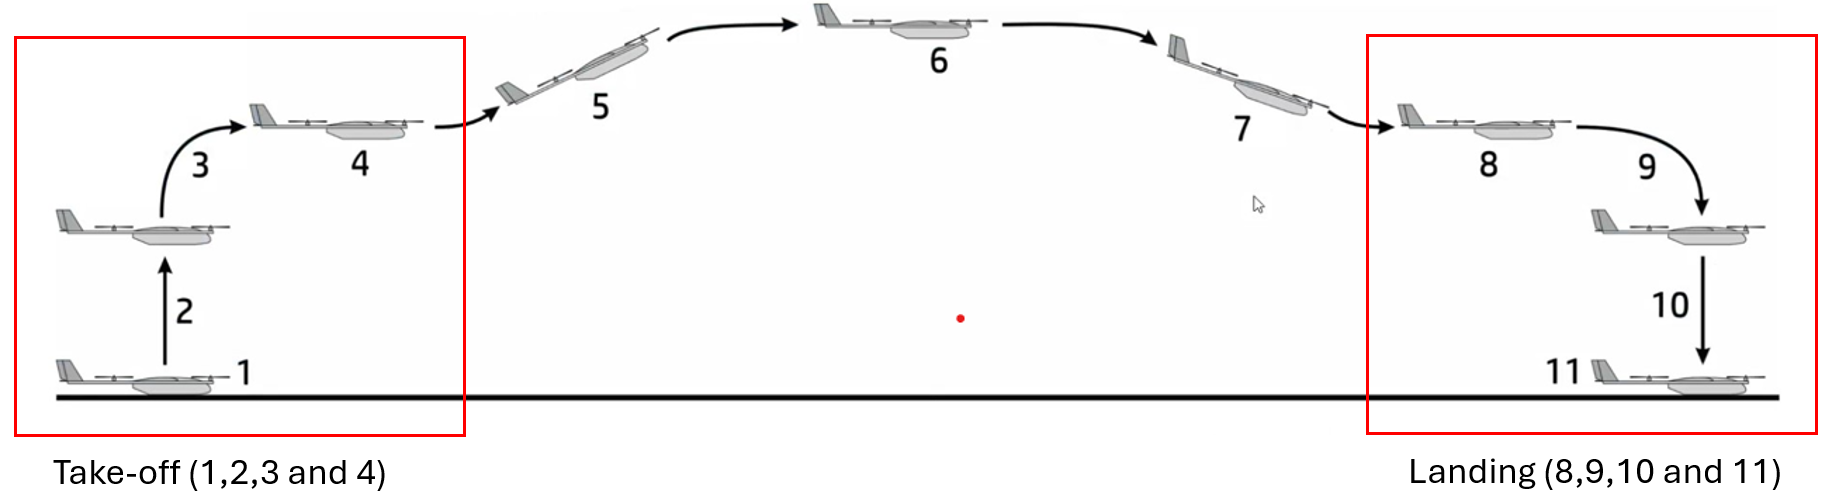
\includegraphics[width=\dimexpr\linewidth-11pt\relax]{images/passos.png}
      \caption{Ilustração das etapas de voo de um VTOL}
      \label{anomalias}
\end{figure}

A partir de curvas de empuxo e torque dos motores, e dos momentos de inércia do VANT, um modelo matemático será desenvolvido e validado com dados de voo reais. Este modelo servirá como base para o desenvolvimento de algoritmos de controle e simulação, visando a criação de um piloto automático para as manobras de decolagem e pouso.

\section{Método M4M de Identificação}

Para a identificação do sistema, foi utilizada a metodologia M4M (Maneuver, Measurements, Methods, Models), uma abordagem estruturada e amplamente utilizada na identificação de sistemas de veículos aéreos [2]. A metodologia M4M divide o processo de identificação em fases bem definidas, garantindo uma abordagem sistemática e robusta.

\begin{figure}
      \centering
      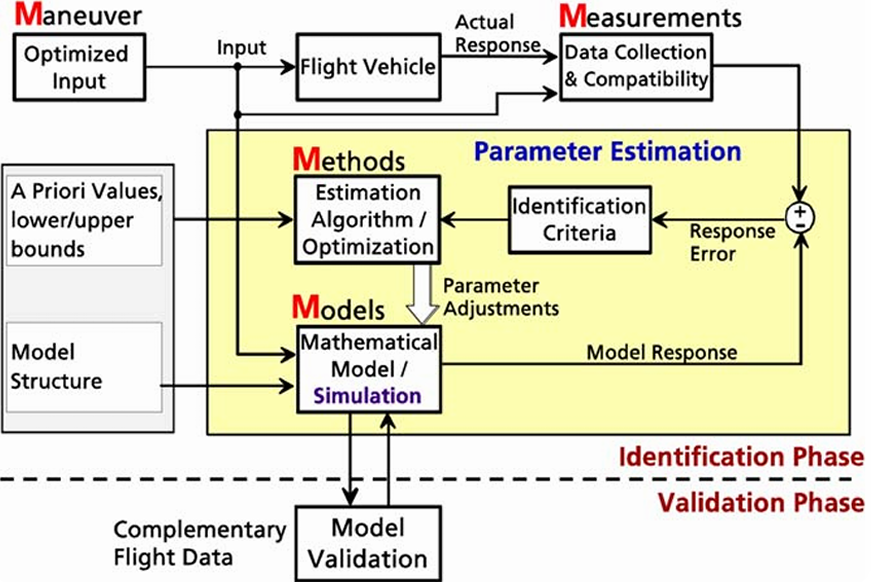
\includegraphics[width=\linewidth]{images/m4m.png}
      \caption{Diagrama do método M4M}
      \label{unet}
\end{figure}


\begin{RaggedRight}
As fases da metodologia M4M são:
\begin{itemize}
    \item \textbf{Maneuver (Manobra):} Entradas otimizadas são projetadas e aplicadas ao veículo em voo para excitar adequadamente a sua dinâmica.
    \item \textbf{Measurements (Medições):} Os dados da resposta real da aeronave às manobras são coletados por meio de sensores embarcados. A compatibilidade e a qualidade dos dados são verificadas nesta fase.
    \item \textbf{Methods (Métodos):} Algoritmos de estimação e otimização são utilizados para identificar os parâmetros do modelo matemático. O ajuste é feito com base em critérios de identificação, em particular na minimização do erro entre resposta real e simulada.
    \item \textbf{Models (Modelos):} Um modelo matemático estrutural, com valores iniciais (a priori), é continuamente refinado com os parâmetros estimados até que o erro seja minimizado.
\end{itemize}
\end{RaggedRight}

Após a fase de identificação, o modelo obtido é submetido a uma fase de validação, na qual dados de voo complementares, não utilizados na estimação, são usados para verificar a capacidade preditiva e a robustez do modelo.

\section{Modelo Matemático do UAV VTOL}

O modelo matemático do VANT VTOL foi desenvolvido considerando a aeronave como um corpo rígido. O modelo unifica a dinâmica tanto para o modo de voo como quadrirotor quanto como asa fixa, e também a fase de transição entre eles.

\begin{figure}
      \centering
      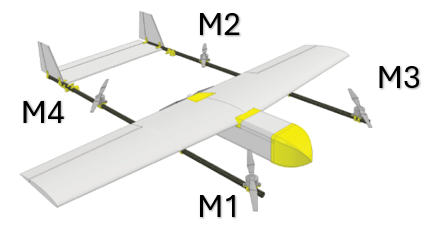
\includegraphics[width=\dimexpr\linewidth-11pt\relax]{images/drone.png}
      \caption{Representação Drone e Motores}
      \label{unet3}
\end{figure}

O modelo é descrito por um conjunto de equações de estado não-lineares. Os vetores de estado ($x$) e de entrada ($u$) são definidos como:
$$
x = [\phi, \theta, \psi, p, q, r, u, v, w, \delta_a, \delta_e, \delta_r]^T
$$
$$
u = [\delta_a^{sp}, \delta_e^{sp}, \delta_r^{sp}, \delta_t, \delta_{MR,1}, \delta_{MR,2}, \delta_{MR,3}, \delta_{MR,4}]^T
$$
Onde $\phi, \theta, \psi$ são os ângulos de Euler; $p, q, r$ são as velocidades angulares; $u, v, w$ são as velocidades lineares no sistema de eixos do corpo; $\delta_a, \delta_e, \delta_r$ são as deflexões das superfícies de controle; $\delta_a^{sp}, \delta_e^{sp}, \delta_r^{sp}$ são os setpoints das superfícies de controle; $\delta_t$ é a entrada do motor de voo de cruzeiro; e $\delta_{MR,i}$ são as entradas dos quatro motores do multirotor [3].

As equações de força no referencial do corpo são dadas por:

\begin{align}
\dot{u} &= rv - qw + \frac{1}{m}(X + T - mg\sin\theta) \\
\dot{v} &= pw - ru + \frac{1}{m}(Y + mg\sin\phi\cos\theta) \\
\dot{w} &= qu - pv + \frac{1}{m}(Z - T_{MR} + mg\cos\phi\cos\theta)
\end{align}

Onde $X, Y, Z$ são as forças aerodinâmicas, $T$ é o empuxo do motor de asa fixa, $T_{MR}$ é o empuxo total dos motores do multirotor e $mg$ é a força da gravidade.

As equações de momento são:
\begin{align}
\dot{p} &= \Gamma_1 pq - \Gamma_2 qr + \Gamma_3 \tau_x + \Gamma_4 \tau_z \\
\dot{q} &= \Gamma_5 pr - \Gamma_6 (p^2 - r^2) + \frac{1}{J_{yy}}\tau_y \\
\dot{r} &= \Gamma_7 pq - \Gamma_1 qr + \Gamma_4 \tau_x + \Gamma_8 \tau_z
\end{align}

Onde $\tau_x, \tau_y, \tau_z$ são os torques totais (aerodinâmicos e dos motores) em torno dos eixos do corpo. As constantes $\Gamma_i$ são funções dos momentos e produtos de inércia ($J_{xx}, J_{yy}, J_{zz}, J_{xz}$) da aeronave [6].

As equações da cinemática dos ângulos de Euler são:

\begin{align}
\dot{\phi} &= p + \tan\theta(q\sin\phi + r\cos\phi) \\
\dot{\theta} &= q\cos\phi - r\sin\phi \\
\dot{\psi} &= \frac{q\sin\phi + r\cos\phi}{\cos\theta}
\end{align}

\section{Modelo do Quadrirotor}
No modo de voo quadrirotor, o controle da aeronave é realizado exclusivamente pelos quatro motores de sustentação [4]. A força de empuxo total $T_{MR}$ gerada pelos motores atua principalmente na direção do eixo $z$ do corpo, controlando a altitude.
$$
F_{MR} = [0, 0, -T_{MR}]^T \quad
$$
Os momentos de controle de rolagem ($\tau_x$), arfagem ($\tau_y$) e guinada ($\tau_z$) são gerados pela variação diferencial do empuxo de cada motor e pelo contra-torque aerodinâmico [5]. Os momentos de rolagem e arfagem são gerados pelo empuxo diferencial dos motores:
$$
\tau_{MR_T} = [\tau_{MR_{T,x}}, \tau_{MR_{T,y}}, 0]^T \quad
$$
O momento de guinada é gerado pelo contra-torque resultante da rotação dos hélices. Motores 1 e 2 giram em um sentido, enquanto os motores 3 e 4 giram no sentido oposto para cancelar o torque em voo pairado [5].
$$
Q_{MR} = Q_{MR,1} + Q_{MR,2} - Q_{MR,3} - Q_{MR,4} \quad
$$

A modelagem da atitude do quadrirotor é frequentemente realizada utilizando ângulos de Euler ou Quatérnions.

\section{Otimização por Mínimos Quadrados Não-Lineares}

A estimação dos parâmetros do modelo matemático foi realizada por meio de um método de otimização de mínimos quadrados não-lineares. Essa abordagem é uma técnica robusta no domínio do tempo, projetada para determinar os parâmetros de um sistema ao minimizar a soma dos quadrados das diferenças entre os dados medidos e a predição de um modelo não-linear. O objetivo central é encontrar um vetor de parâmetros $\Theta$ que minimize a função de custo, que representa o erro residual entre a saída real do sistema, $z$, e a saída simulada pelo modelo, $y(\Theta)$.

O processo de otimização pode ser resumido nas seguintes etapas:
\begin{itemize}
    \item Uma entrada de controle conhecida ($u$) é aplicada tanto ao veículo aéreo real quanto ao modelo matemático que se deseja identificar.
    \item A resposta do sistema real ($z$) a essa entrada é registrada pelos sensores da aeronave, sendo sujeita a ruídos de medição inerentes ao processo.
    \item O modelo matemático, implementado computacionalmente, utiliza a mesma entrada ($u$) para simular a resposta do sistema ($y$) com base em um conjunto inicial de parâmetros $\Theta$.
    \item O resíduo, ou erro de resposta (z-y), é calculado em cada ponto no tempo.
    \item Um algoritmo de otimização ajusta iterativamente os parâmetros $\Theta$ do modelo com o objetivo de minimizar a soma dos quadrados dos resíduos. Este processo continua até que os critérios de convergência sejam atendidos. [2].
\end{itemize}

A função de custo a ser minimizada é dada por:
\begin{align}
J(\Theta) = {} & \sum_{k=1}^{N} [z(t_{k}) - y(t_{k},\Theta)] = \sum_{k=1}^{N} f_{k}(\Theta)^2
\end{align}

Onde $f_{k}(\Theta)$ representa o erro residual no instante de tempo $t_{k}$. O problema de otimização consiste em encontrar:

\begin{align}
min_{\Theta} \frac{1}{2}\|f(\theta)\|_{2}^2 = \frac{1}{2}sum_{k=1}^{N} f_{k}(\Theta)^2
\end{align}

O processo de atualização dos parâmetros, conduzido por algoritmos como o de Levenberg-Marquardt, é um ciclo iterativo fundamentado na sensibilidade do erro do modelo em relação a cada parâmetro. A cada iteração $k$, o objetivo é encontrar um vetor de atualização, $\delta_k$, que, ao ser somado ao vetor de parâmetros atual, $\Theta_k$, produza um novo vetor $\Theta_{k+1 }$ que reduza o valor da função de custo.

Para determinar a direção e a magnitude ideais desse passo, o algoritmo primeiro calcula a matriz Jacobiana, J. A Jacobiana é uma matriz que contém as derivadas parciais de primeira ordem de cada componente do vetor de erro residual em relação a cada parâmetro do modelo. Essencialmente, ela quantifica a sensibilidade da saída do sistema a pequenas alterações nos parâmetros:

\begin{align}
J_{ij} = \frac{\partial f(\Theta)}{\partial \Theta_j}
\end{align}

O método de Levenberg-Marquardt utiliza a Jacobiana para calcular o passo de atualização $\delta$ através da solução do seguinte sistema de equações lineares:

\begin{align}
(J^TJ + \lambda I)\delta = -J^T f(\Theta)
\end{align}

Após resolver o sistema e encontrar o vetor de passo $\delta_k$, os parâmetros são atualizados pela seguinte regra:

\begin{align}
\Theta_{k+1} = \Theta_{k} + \delta_k
\end{align}

\section{Metodologia}

A abordagem metodológica deste trabalho é fundamentada na estrutura de identificação de sistemas M4M (Maneuver, Measurements, Methods, Models). Essa metodologia provê um caminho sistemático para a obtenção de modelos matemáticos a partir de dados experimentais. As etapas práticas envolveram a coleta de dados de voo através de manobras específicas, a determinação de constantes iniciais para o modelo e a implementação do modelo matemático em um ambiente de simulação para o processo de identificação

\subsection{Manobras e Dados para Identificação}

A qualidade da identificação de sistema depende diretamente da qualidade dos dados coletados. Para garantir que os dados contivessem informação suficiente sobre a dinâmica da aeronave, foram executadas manobras de voo especificamente projetadas para excitar os modos de movimento do VANT em torno de seus eixos principais: rolagem, arfagem e guinada (Roll, Pitch, Yaw) [7] [8].

Os dados para o processo de identificação foram extraídos diretamente dos logs de voo da aeronave [9]. Esses dados foram divididos em dois conjuntos principais:

\begin{sloppypar}
\begin{itemize}
    \item \textbf{Entradas do Sistema (u):} Correspondem aos sinais de controle enviados aos atuadores da aeronave. Para o modo de voo multirotor, as entradas são os sinais de Modulação por Largura de Pulso (PWM) que comandam a velocidade de rotação de cada um dos quatro motores. Esses sinais foram registrados ao longo do tempo durante as manobras.
    \item \textbf{Saídas do Sistema (y):} Correspondem à resposta da aeronave às entradas de controle, medidas pelos sensores embarcados. As saídas utilizadas para a identificação da atitude foram as velocidades angulares nos eixos do corpo: velocidade de rolagem (p), arfagem (q) e guinada (r). Estas foram medidas em radianos por segundo.
\end{itemize}
\end{sloppypar}

\begin{figure}
      \centering
      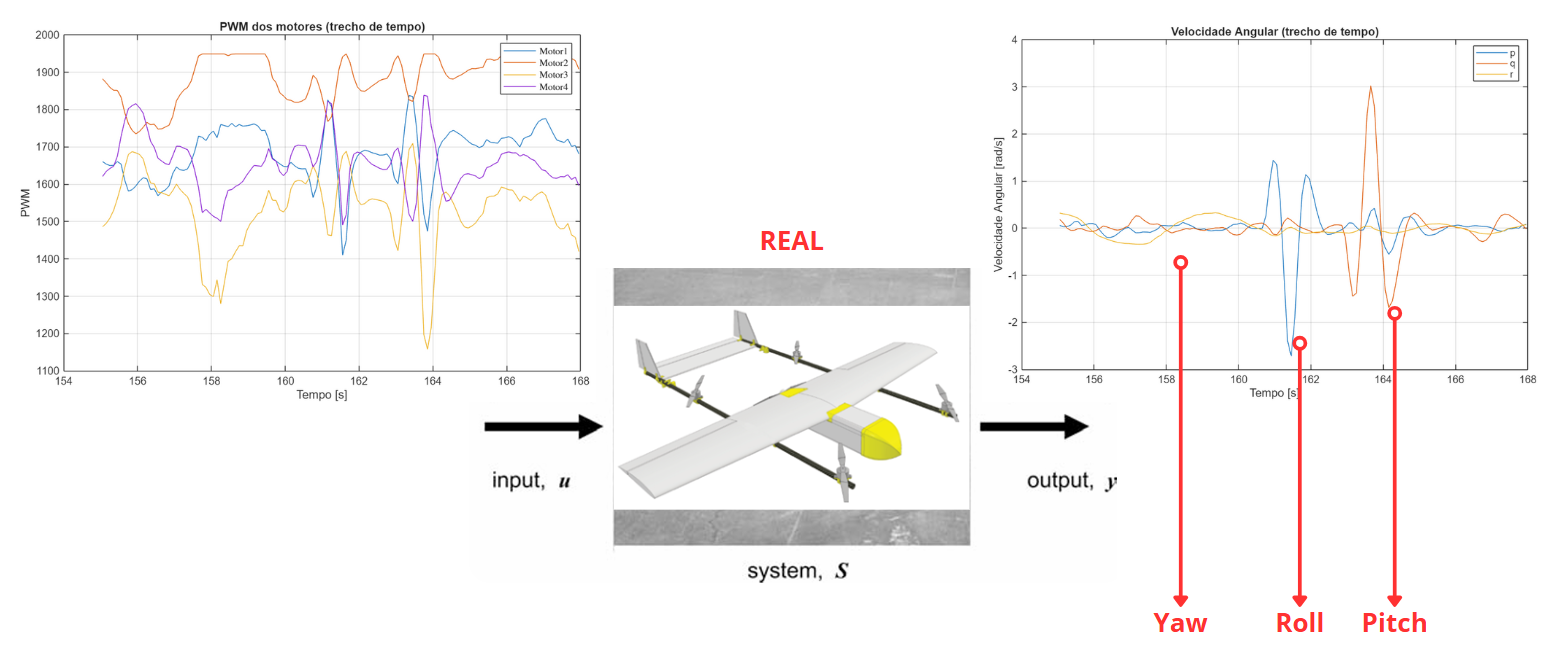
\includegraphics[width=\linewidth]{images/measurements.png}
      \caption{Dados de Identificação}
\end{figure}

\subsection{Constantes Iniciais}
\begin{sloppypar}
As constantes iniciais do modelo, como parâmetros geométricos, massa e momentos de inércia, foram obtidas por meio de medições físicas da aeronave e dados de campanhas de voo anteriores. Alguns dos principais parâmetros são apresentados na tabela a seguir [10].
\end{sloppypar}

\begin{table}[htbp]
\centering
\begin{tabular}{l|c|c|l}
\hline
\textbf{Parâmetro} & \textbf{Valor} & \textbf{Unidade} & \textbf{Modo de obtenção} \\
\hline
$S$ & 0.27 & m$^2$ & Medição física \\
$b$ & 1,20 & m & Medição física \\
$c$ & 0,226 & m & Medição física \\
$m_{total}$ & 2,20 & kg & Medição física com balanças \\
$\alpha_{trim}$ & 0 & rad & Medição física \\
\hline
\end{tabular}
\caption{Parâmetros físicos e de voo do VANT.}
\end{table}

Os coeficientes aerodinâmicos foram obtidos de simulações e dados de voo.

\subsection{Simulação Dinâmica do Modelo}

O conjunto completo de equações diferenciais não-lineares que descreve a dinâmica de corpo rígido do VANT foi implementado em um modelo de simulação. O ambiente MATLAB/Simulink foi escolhido para esta tarefa, dada sua ampla utilização e robustez na simulação de sistemas dinâmicos complexos.

O modelo em Simulink, nomeado "Hybrid Drone Model", representa fielmente a estrutura matemática do sistema. Ele foi estruturado em blocos que calculam as forças e momentos (aerodinâmicos e de propulsão), integram as equações de movimento para obter as velocidades, e integram as equações cinemáticas para obter a atitude.

Esta simulação é o coração do método de estimação: ela gera a resposta prevista do modelo (y) para uma dada entrada. Essa resposta prevista é então comparada com a resposta real da aeronave (z) para calcular o erro que o algoritmo de otimização irá minimizar.

\begin{figure}
      \centering
      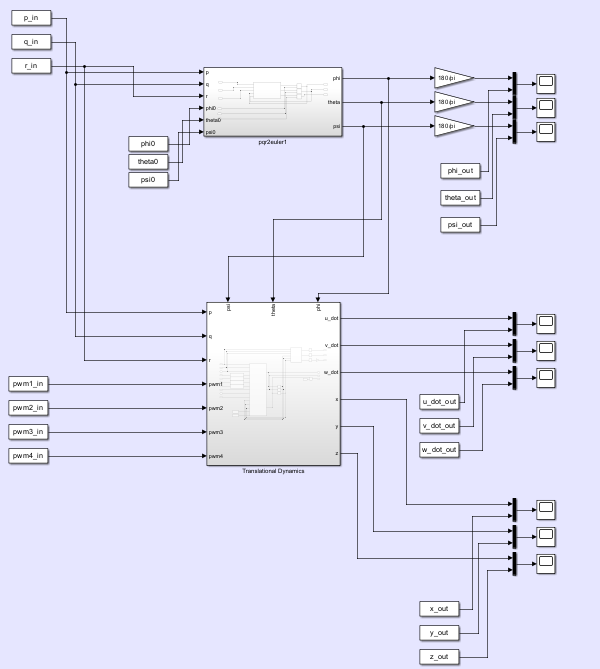
\includegraphics[width=8.5cm]{images/simu.png}
      \caption{Simulação via Simulink do Modelo}
      \label{decoder}
\end{figure}

\begin{figure}
      \centering
      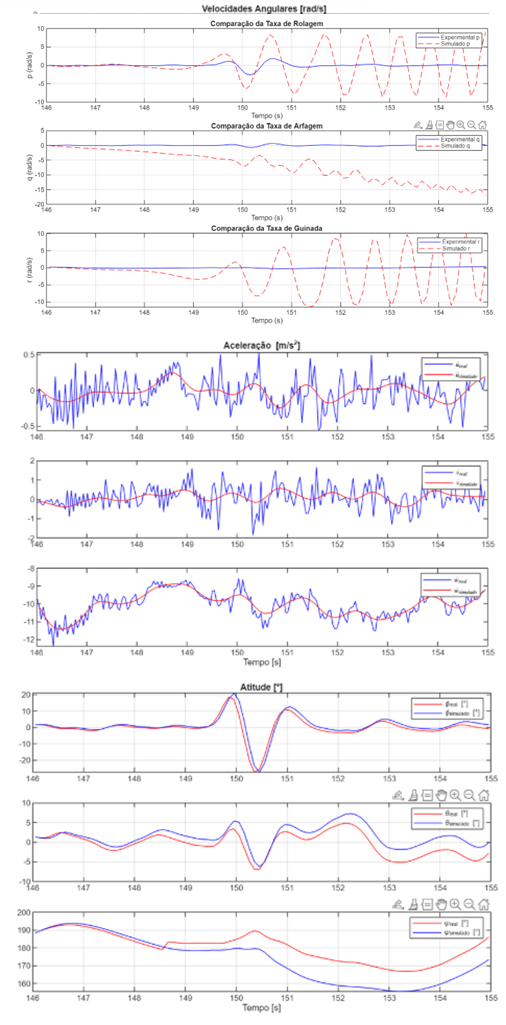
\includegraphics[width=7cm]{images/Imagem1.png}
      \caption{Validação da Identificação}
      \label{loss}
\end{figure}


\section{RESULTADO E DISCUSSÕES}

A aplicação do método dos mínimos quadrados a um sistema não linear com dados de voo permitiu a estimação dos parâmetros do modelo matemático.

\subsection{Resultado da Estimação dos Parâmetros}

O processo de otimização resultou em um conjunto de parâmetros estimados para as constantes de inércia e para os coeficientes de empuxo e torque dos motores. Os parâmetros estimados são apresentados abaixo.

\begin{table}[htbp]
\centering
\begin{tabular}{l|c}
\hline
\textbf{Parâmetro} & \textbf{Valor Estimado} \\
\hline
G1 & 0.0043426 \\
G2 & -0.65222 \\
G3 & 23.1355 \\
G4 & 0.28798 \\
G5 & 0.53723 \\
G6 & 0.010112 \\
G7 & -0.88082 \\
G8 & 7.9277 \\
InvJy & 6.4763 \\
k\_T1 & 0.60007 \\
k\_T2 & 0.44999 \\
k\_T3 & 1 \\
k\_T4 & 0.80002 \\
k\_Q1 & 0.60001 \\
k\_Q2 & 0.45 \\
k\_Q3 & 1 \\
k\_Q4 & 0.79994 \\
\hline
\end{tabular}
\caption{Parâmetros estimados.}
\end{table}

\subsection{Validação}
A validação do modelo identificado foi realizada comparando a resposta simulada com um conjunto de dados de voo real que não foi utilizado no processo de estimação. Os gráficos abaixo mostram a comparação entre os dados reais (em azul) e os dados simulados pelo modelo (em vermelho) para os ângulos de atitude (rolagem, arfagem e guinada).


Os resultados da validação demonstram uma excelente aderência entre a resposta do modelo identificado e os dados reais de voo, indicando que o modelo matemático captura com precisão a dinâmica da aeronave. A boa correspondência entre as curvas valida a eficácia da metodologia de identificação empregada.

\section{CONCLUSÃO}

Este trabalho apresentou o processo de modelagem e identificação de sistema de um VANT VTOL híbrido. Utilizando a metodologia M4M e o método de estimação dos mínimos quadrados em um sistema não-linear, foi possível desenvolver um modelo matemático não-linear que representa com certa fidelidade o comportamento dinâmico da aeronave.

As constantes iniciais foram obtidas a partir de medições físicas e dados prévios, e os parâmetros aerodinâmicos e de inércia foram refinados através do processo de identificação com dados de voo reais. A validação do modelo com um conjunto de dados distinto demonstrou a sua precisão e robustez.

O modelo matemático validado constitui uma ferramenta essencial para os próximos passos do projeto, que incluem o projeto de sistemas de controle avançados e o desenvolvimento de um piloto automático capaz de realizar de forma autônoma as manobras de decolagem, transição e pouso, cumprindo assim os objetivos principais do projeto.

\addtolength{\textheight}{-12cm}   % This command serves to balance the column lengths
                                  % on the last page of the document manually. It shortens
                                  % the textheight of the last page by a suitable amount.
                                  % This command does not take effect until the next page
                                  % so it should come on the page before the last. Make
                                  % sure that you do not shorten the textheight too much.

%%%%%%%%%%%%%%%%%%%%%%%%%%%%%%%%%%%%%%%%%%%%%%%%%%%%%%%%%%%%%%%%%%%%%%%%%%%%%%%%



%%%%%%%%%%%%%%%%%%%%%%%%%%%%%%%%%%%%%%%%%%%%%%%%%%%%%%%%%%%%%%%%%%%%%%%%%%%%%%%%



%%%%%%%%%%%%%%%%%%%%%%%%%%%%%%%%%%%%%%%%%%%%%%%%%%%%%%%%%%%%%%%%%%%%%%%%%%%%%%%%

%%%%%%%%%%%%%%%%%%%%%%%%%%%%%%%%%%%%%%%%%%%%%%%%%%%%%%%%%%%%%%%%%%%%%%%%%%%%%%%%


\begin{thebibliography}{99}

\bibitem{c1} Vladislav Klein and Eugene A. Morelli. Aircraft System Identification: Theory and Practice. 2006. doi: 10.2514/4.861505.

\bibitem{c2} Ravindra V. Jategaonkar. Flight Vehicle System Identification: A Time Domain Methodology. 2006. isbn: 1563478366.

\bibitem{c3} Mark B. Tischler and Robert K. Remple. Aircraft and Rotorcraft System Identication, Second Edition. 2012. doi: 10.2514/4.868207.

\bibitem{c4} Nathan V. Ho er et al. A survey and categorization of small low-cost unmanned aerial vehicle system identification . In: Journal of Intelligent and Robotic Systems: Theory and Applications 74.1-2 (2014), pp. 129145. issn: 09210296. doi: 10.1007/s10846-013-9931-6.

\bibitem{c5} Ony Ari anto and Mazen Farhood. Development and Modeling of a Low-Cost Unmanned Aerial Vehicle Research Platform. In: Journal of Intelligent and Robotic Systems: Theory and Applications 80.1 (Oct. 2015), pp. 139164. issn: 15730409. doi: 10.1007/s10846-014-0145-3.

\bibitem{c6} MWGreen. Measurement of the moments of inertia of full scale airplanes. Tech. rep. NACA-TN-265. 1927.

\bibitem{c7} David J. Grymin and Mazen Farhood. Two-Step System Identification and Trajectory Tracking Control of a Small Fixed-Wing UAV. In: Journal of Intelli gent and Robotic Systems: Theory and Applications 83.1 (2016). issn: 15730409. doi: 10.1007/s10846-015-0298-8.

\bibitem{c8} Samir Bouabdallah and Roland Siegwart. Full control of a quadrotor. In: IEEE International Conference on Intelligent Robots and Systems October (2007), pp. 153158. issn: 18172172. doi: 10.1109/\allowbreak IROS.2007.4399042.

\bibitem{c9} Daniel Mellinger and Vijay Kumar. Minimum snap trajectory generation and control for quadrotors. In: 2011. isbn: 9781612843865. doi: 10.1109/\allowbreak ICRA.2011.5980409.

\bibitem{c10} S. Verling et al. Full Attitude Control of a VTOL tailsitter UAV. In: Proceed ings- IEEE International Conference on Robotics and Automation 2016-June (2016), pp. 3006 3012. issn: 10504729. doi: 10.1109/ICRA.2016.7487466.

\bibitem{c11} Bernhard P. Graesdal. Full Nonlinear System Identification for a Vertical-Takeoff-and-Landing Unmanned Aerial Vehicle.  Master’s thesis in Cybernetics and Robotics (2022), Norwegian University of Science and Technology

\bibitem{c12} Lawrence E. Hale, Mayuresh Patil, and Christopher J. Roy. Aerodynamic parameter identification and uncertainty quantication for small unmanned air craft . In: Journal of Guidance, Control, and Dynamics. Vol. 40. 3. 2017. doi: 10.2514/1.G000582.

\end{thebibliography}

\end{document}